\documentclass[]{article}
\usepackage{lmodern}
\usepackage{amssymb,amsmath}
\usepackage{ifxetex,ifluatex}
\usepackage{fixltx2e} % provides \textsubscript
\ifnum 0\ifxetex 1\fi\ifluatex 1\fi=0 % if pdftex
  \usepackage[T1]{fontenc}
  \usepackage[utf8]{inputenc}
\else % if luatex or xelatex
  \ifxetex
    \usepackage{mathspec}
  \else
    \usepackage{fontspec}
  \fi
  \defaultfontfeatures{Ligatures=TeX,Scale=MatchLowercase}
\fi
% use upquote if available, for straight quotes in verbatim environments
\IfFileExists{upquote.sty}{\usepackage{upquote}}{}
% use microtype if available
\IfFileExists{microtype.sty}{%
\usepackage{microtype}
\UseMicrotypeSet[protrusion]{basicmath} % disable protrusion for tt fonts
}{}
\usepackage[margin=1in]{geometry}
\usepackage{hyperref}
\hypersetup{unicode=true,
            pdftitle={moretrees: an R package to fit Multi-Outcome Regression with Tree-Structured Shrinkage models via variational inference},
            pdfauthor={Emma Thomas},
            pdfborder={0 0 0},
            breaklinks=true}
\urlstyle{same}  % don't use monospace font for urls
\usepackage{color}
\usepackage{fancyvrb}
\newcommand{\VerbBar}{|}
\newcommand{\VERB}{\Verb[commandchars=\\\{\}]}
\DefineVerbatimEnvironment{Highlighting}{Verbatim}{commandchars=\\\{\}}
% Add ',fontsize=\small' for more characters per line
\usepackage{framed}
\definecolor{shadecolor}{RGB}{248,248,248}
\newenvironment{Shaded}{\begin{snugshade}}{\end{snugshade}}
\newcommand{\AlertTok}[1]{\textcolor[rgb]{0.94,0.16,0.16}{#1}}
\newcommand{\AnnotationTok}[1]{\textcolor[rgb]{0.56,0.35,0.01}{\textbf{\textit{#1}}}}
\newcommand{\AttributeTok}[1]{\textcolor[rgb]{0.77,0.63,0.00}{#1}}
\newcommand{\BaseNTok}[1]{\textcolor[rgb]{0.00,0.00,0.81}{#1}}
\newcommand{\BuiltInTok}[1]{#1}
\newcommand{\CharTok}[1]{\textcolor[rgb]{0.31,0.60,0.02}{#1}}
\newcommand{\CommentTok}[1]{\textcolor[rgb]{0.56,0.35,0.01}{\textit{#1}}}
\newcommand{\CommentVarTok}[1]{\textcolor[rgb]{0.56,0.35,0.01}{\textbf{\textit{#1}}}}
\newcommand{\ConstantTok}[1]{\textcolor[rgb]{0.00,0.00,0.00}{#1}}
\newcommand{\ControlFlowTok}[1]{\textcolor[rgb]{0.13,0.29,0.53}{\textbf{#1}}}
\newcommand{\DataTypeTok}[1]{\textcolor[rgb]{0.13,0.29,0.53}{#1}}
\newcommand{\DecValTok}[1]{\textcolor[rgb]{0.00,0.00,0.81}{#1}}
\newcommand{\DocumentationTok}[1]{\textcolor[rgb]{0.56,0.35,0.01}{\textbf{\textit{#1}}}}
\newcommand{\ErrorTok}[1]{\textcolor[rgb]{0.64,0.00,0.00}{\textbf{#1}}}
\newcommand{\ExtensionTok}[1]{#1}
\newcommand{\FloatTok}[1]{\textcolor[rgb]{0.00,0.00,0.81}{#1}}
\newcommand{\FunctionTok}[1]{\textcolor[rgb]{0.00,0.00,0.00}{#1}}
\newcommand{\ImportTok}[1]{#1}
\newcommand{\InformationTok}[1]{\textcolor[rgb]{0.56,0.35,0.01}{\textbf{\textit{#1}}}}
\newcommand{\KeywordTok}[1]{\textcolor[rgb]{0.13,0.29,0.53}{\textbf{#1}}}
\newcommand{\NormalTok}[1]{#1}
\newcommand{\OperatorTok}[1]{\textcolor[rgb]{0.81,0.36,0.00}{\textbf{#1}}}
\newcommand{\OtherTok}[1]{\textcolor[rgb]{0.56,0.35,0.01}{#1}}
\newcommand{\PreprocessorTok}[1]{\textcolor[rgb]{0.56,0.35,0.01}{\textit{#1}}}
\newcommand{\RegionMarkerTok}[1]{#1}
\newcommand{\SpecialCharTok}[1]{\textcolor[rgb]{0.00,0.00,0.00}{#1}}
\newcommand{\SpecialStringTok}[1]{\textcolor[rgb]{0.31,0.60,0.02}{#1}}
\newcommand{\StringTok}[1]{\textcolor[rgb]{0.31,0.60,0.02}{#1}}
\newcommand{\VariableTok}[1]{\textcolor[rgb]{0.00,0.00,0.00}{#1}}
\newcommand{\VerbatimStringTok}[1]{\textcolor[rgb]{0.31,0.60,0.02}{#1}}
\newcommand{\WarningTok}[1]{\textcolor[rgb]{0.56,0.35,0.01}{\textbf{\textit{#1}}}}
\usepackage{longtable,booktabs}
\usepackage{graphicx,grffile}
\makeatletter
\def\maxwidth{\ifdim\Gin@nat@width>\linewidth\linewidth\else\Gin@nat@width\fi}
\def\maxheight{\ifdim\Gin@nat@height>\textheight\textheight\else\Gin@nat@height\fi}
\makeatother
% Scale images if necessary, so that they will not overflow the page
% margins by default, and it is still possible to overwrite the defaults
% using explicit options in \includegraphics[width, height, ...]{}
\setkeys{Gin}{width=\maxwidth,height=\maxheight,keepaspectratio}
\IfFileExists{parskip.sty}{%
\usepackage{parskip}
}{% else
\setlength{\parindent}{0pt}
\setlength{\parskip}{6pt plus 2pt minus 1pt}
}
\setlength{\emergencystretch}{3em}  % prevent overfull lines
\providecommand{\tightlist}{%
  \setlength{\itemsep}{0pt}\setlength{\parskip}{0pt}}
\setcounter{secnumdepth}{5}
% Redefines (sub)paragraphs to behave more like sections
\ifx\paragraph\undefined\else
\let\oldparagraph\paragraph
\renewcommand{\paragraph}[1]{\oldparagraph{#1}\mbox{}}
\fi
\ifx\subparagraph\undefined\else
\let\oldsubparagraph\subparagraph
\renewcommand{\subparagraph}[1]{\oldsubparagraph{#1}\mbox{}}
\fi

%%% Use protect on footnotes to avoid problems with footnotes in titles
\let\rmarkdownfootnote\footnote%
\def\footnote{\protect\rmarkdownfootnote}

%%% Change title format to be more compact
\usepackage{titling}

% Create subtitle command for use in maketitle
\providecommand{\subtitle}[1]{
  \posttitle{
    \begin{center}\large#1\end{center}
    }
}

\setlength{\droptitle}{-2em}

  \title{moretrees: an R package to fit Multi-Outcome Regression with
Tree-Structured Shrinkage models via variational inference}
    \pretitle{\vspace{\droptitle}\centering\huge}
  \posttitle{\par}
    \author{Emma Thomas}
    \preauthor{\centering\large\emph}
  \postauthor{\par}
      \predate{\centering\large\emph}
  \postdate{\par}
    \date{2020-04-21}


\begin{document}
\maketitle

\hypertarget{intro}{%
\section{Introduction}\label{intro}}

The \texttt{moretrees} package fits Multi-Outcome Regression with
Tree-structured Shrinkage (MOReTreeS) models to case-crossover and
matched case-control data when being a `case' can mean experiencing one
of multiple related outcomes. MOReTreeS models require that these
outcomes are related according to a known tree. For example, the
outcomes might be multiple distinct cardiovascular diseases that can be
labelled using a hierarchical, tree-like classification system, as in
the worked example in Section 3 below.

The MOReTreeS model simultaneously achieves three core functions:

\begin{enumerate}
\def\labelenumi{\arabic{enumi}.}
\tightlist
\item
  discovers \emph{de novo} groups of outcomes that have a similar
  association with the exposure conditional on matching factors and
  covariates, with both the number and composition of the groups
  estimated from the data;
\item
  estimates a group-specific measure of association with the exposure
  for each outcome group;
\item
  performs \texttt{information\ sharing} across the outcomes by
  shrinking the coefficient estimates for different outcomes towards
  each other, with the degree of shrinkage determined by how closely
  related those outcomes are on the tree.
\end{enumerate}

The model is fit using variational inference (VI), a fast alternative to
Markov chain Monte Carlo (MCMC) for approximating posterior
distributions of Bayesian models.

This vignette is divided into three sections. Section 2 provides details
of the MOReTreeS model implemented by the package. Section 3 lays out
the functionality of the \texttt{moretrees} package in a readable form
and guides potential users through an example of fitting the model using
the \texttt{moretrees()} function. Finally, Section 4 explains the VI
algorithm used to fit the model. Section 4 is not essential reading for
most users, but rather aims to provide sufficient detail about the
algorithm that someone with knowledge of VI would be able to write their
own code to fit the model.

\hypertarget{model}{%
\section{Model details}\label{model}}

We begin by giving details of the model implemented by the
\texttt{moretrees} package. The model is very similar to the one
presented in Thomas et al. (2020), with extensions to allow for: (1) a
multivariate exposure; (2) control for covariates in regression
analyses, and; (3) more flexible hyperparameter specification. MOReTreeS
priors can be used with a range of different outcome distributions or
likelihoods; the \texttt{moretrees()} function implements the
conditional logistic likelihood used in conditional logistic regression
(CLR) analyses, the standard method for both matched case-control
studies and case-crossover studies. We first define the CLR likelihood
used in our study, and then the MOReTreeS prior.

\hypertarget{likelihood}{%
\subsection{Likelihood}\label{likelihood}}

Let \(\mathcal{V}\) be the set of outcomes under study. For outcome
\(v\) in \(\mathcal{V}\), let \(Y_{i,j}^{(v)}\) be a binary variable
indicating whether a hospitalization for disease \(v\) occurred on day
\(j\) for individual \(i\), where without loss of generality we assume
\(j = 1\) represents the case day and \(j = 2\) represents the control
day. Let \(\mathbf{x}_{i,j}^{(v)}\) be the exposure vector of length
\(k\) and \(\mathbf{w}_{i,j}^{(v)}\) be a vector of covariates of length
\(m\). For notational convenience, we let
\(\mathbf{x}_i^{(v)} = \mathbf{x}_{i,1}^{(v)} - \mathbf{x}_{i,2}^{(v)}\)
and
\(\mathbf{w}_i^{(v)} = \mathbf{w}_{i,1}^{(v)} - \mathbf{w}_{i,2}^{(v)}\).

The conditional logistic likelihood for each matched pair is shown below
(Maclure 1991).

\begin{equation}
\tag{1}
P\left(Y_{i,1}^{(v)} = 1, Y_{i,2}^{(v)} = 0 \middle\vert Y_{i,1}^{(v)} + Y_{i,2}^{(v)} = 1, \boldsymbol{\beta}_v, \boldsymbol{\theta}_v \right) = \textrm{logit} \left( \boldsymbol{\beta}_v^T \mathbf{x}_{i}^{(v)} + \boldsymbol{\theta}_v^T \mathbf{w}_i^{(v)} \right).
\end{equation}

where \(\boldsymbol{\beta}\) is the coefficient vector for the effect of
the exposure on outcome \(v\), \(\boldsymbol{\theta}_v\) is the vector
of covariate effects for outcome \(v\), and
\(\textrm{logit}(y) = 1 / (1+ e^{-y})\) is the logistic or sigmoid
function. The full data likelihood is obtained by multiplying over all
matched pairs.

\hypertarget{prior}{%
\subsection{Prior}\label{prior}}

The MOReTreeS spike and slab prior enables data-driven discovery of
groups of outcomes that have a similar relationship with PM\(_{2.5}\)
(Thomas et al. 2020). Let \(\mathcal{V}\) be the set of nodes on the
tree of outcome relationships, and let
\(\mathcal{V}_L \subset \mathcal{V}\) be the set of leaves. Internal
nodes \(u \in \mathcal{V}\) represent outcome categories and leaf nodes
\(v \in \mathcal{V}_L\) represent individual outcomes. Let \(a(v)\) be
the set of ancestors nodes of \(v \in \mathcal{V}_L\), including \(v\)
itself. Finally, let \(l_u \in \lbrace 1, \dots, L \rbrace\) indicate
which hyperparameters apply to variables at node \(u \in \mathcal{V}\)
on the tree. We explain below what is meant by this.

The prior is:

\begin{align*}
\boldsymbol{\beta}_v & = \sum_{u \in a(v)} s_u \boldsymbol{\gamma}_u \\
\boldsymbol{\theta}_v & = \sum_{u \in a(v)} \boldsymbol{\zeta}_u \\
s_u & \sim Bern(\rho_{l_u}) \\
\boldsymbol{\gamma}_u & \sim \mathcal{MVN}\left(\boldsymbol{0},\tau_{l_u} I_k\right) \\
\boldsymbol{\zeta}_u & \sim \mathcal{MVN} \left( \boldsymbol{0}, \omega_{l_u} I_m \right) \\
\rho_{l} & \sim Beta(a_l, b_l).
\end{align*}

Here the `node parameters' \(s_u \boldsymbol{\gamma}_u\) and
\(\boldsymbol{\zeta}_u\) can be interpreted as the difference in the
exposure effect for outcome category \(u\) compared to its parent
category. \(\rho_l\), \(\tau_l\), and \(\omega_l\) for
\(l = 1, \dots, L\) are hyperparameters representing, respectively, the
prior probability of inclusion for node parameters
\(\boldsymbol{\gamma}_u\), the prior variance of all elements of
\(\boldsymbol{\gamma}_u\), and the prior variance of all elements of
\(\boldsymbol{\zeta}_u\) for \(u\) such that \(l_u = u\). The \(l_u\)
are fixed values from 1 through \(L\) that specify which nodes on the
tree share common hyperparameters \(\rho_l\), \(\tau_l\), and
\(\omega_l\). The default used by \texttt{moretrees()} is to have two
sets of hyperparameters: one for all internal nodes (\(l_u = 1\) for
\(u \in \mathcal{V} \backslash \mathcal{V}_L\)), and one for all leaf
nodes (\(l_u = 2\) for \(u \in \mathcal{V}_L\)). \(\tau_l\) and
\(\omega_l\) are estimated via approximate empirical Bayes as discussed
below in Section 4.4; we place a conditionally conjugate beta hyperprior
on \(\rho_l\).

The above hierarchical model leads to the formation of groups of
outcomes with the same exposure effects by fusing (setting equal)
coefficients for different outcomes. This fusion process is achieved as
follows. The coefficients \(\boldsymbol{\beta}_{v_1}\) and
\(\boldsymbol{\beta}_{v_2}\) for any two outcomes
\(v_1, v_2 \in \mathcal{V}_L\) will be exactly equal if and only if
\(s_u = 0\) for all \(u \in d(v_1, v_2)\), where
\(d(v_1, v_2) = (a(v_1) \cup a(v_2)) \backslash (a(v_1) \cap a(v_2))\)
is the set of nodes that are ancestors of either \(v_1\) or \(v_2\) but
not both. The result is that the prior probability that
\(\boldsymbol{\beta}_{v_1}\) and \(\boldsymbol{\beta}_{v_2}\) are equal,
meaning \(v_1\) and \(v_2\) are grouped together, depends on both on the
set of nodes \(d(v_1, v_2)\) that `separate' the two leaf nodes \(v_1\)
and \(v_2\) on the tree, as well as on the hyperparameters \(\rho_l\).
Specifically, conditional on the \(\rho_l\),

\[P\left(\mathbf{\beta}_{v_1} = \mathbf{\beta}_{v_2} \vert \rho_1, \dots, \rho_L \right) = \prod_{l=1}^L (1 - \rho_l)^{\left\vert d(v_1, v_2) \cap \lbrace u: l_u = l \rbrace \right\vert}.\]
Let
\(n(v_1, v_2, l) = \left\vert d(v_1, v_2) \cap \lbrace u: l_u = l \rbrace \right\vert\).
Integrating over the parameters \(\rho_l\), we find:

\[P\left(\mathbf{\beta}_{v_1} = \mathbf{\beta}_{v_2}\right) = \prod_{l = 1}^L \left(\prod_{r = 0}^{n(v_1,v_2,l)} \dfrac{b_l + r}{a_l + b_l + r}\right)^{\mathbf{1}_{n > 0}\left(n(v_1,v_2,l)\right)}. \]
This expression can be derived using the higher moments of the Beta
distribution.

\hypertarget{posterior-estimates}{%
\subsection{Posterior estimates}\label{posterior-estimates}}

\texttt{moretrees} obtains posterior estimates for the exposure effects
\(\boldsymbol{\beta}_v\) in the same manner as described by Thomas et
al. (2020). Briefly, the \texttt{moretrees()} function returns estimates
from the \emph{median probability model} that includes only those node
variables with marginal posterior inclusion probability greater than 0.5
(Barbieri and Berger 2004). As discussed in the previous section, a node
is included in the model if \(s_u = 1\). Thus, a node will be included
in our final model if the posterior probability that \(s_u = 1\) is
greater than 0.5.

\hypertarget{code}{%
\section{\texorpdfstring{\texttt{moretrees()}: functionality and
usage}{moretrees(): functionality and usage}}\label{code}}

\hypertarget{functionality}{%
\subsection{Functionality}\label{functionality}}

The \texttt{moretrees()} function fits MOReTrees models and supports the
following functionality:

\begin{enumerate}
\def\labelenumi{\arabic{enumi}.}
\tightlist
\item
  Fitting MOReTreeS models to pair matched case-control or
  case-crossover data where each case is associated with exactly one
  outcome among a set of related outcomes;
\item
  Multiple exposure types: \texttt{moretrees()} supports any exposure
  type by supplying appropriate design matrices for the cases and
  controls;
\item
  Control for confounding in regression model: confounders which could
  not be matched on can be controlled for in the regression model;
  information about covariate effect sizes will be shared across the
  outcomes;
\item
  Hyperparameter selection: the user need not specify the values of
  hyperparameters which are instead estimated via an approximate
  empirial Bayes scheme, as detailed in Section 4.4.
\end{enumerate}

\hypertarget{worked-example}{%
\subsection{Worked example}\label{worked-example}}

We illustrate use of the \texttt{moretrees()} function with a small
simulated dataset, \texttt{moretreesCaseCrossover}, which has
\(n = 1000\) case-crossover pairs, \(p = 11\) outcomes, an exposure with
dimension \(k = 2\), and \(m = 2\) covariates. The data are stored as a
list with the following elements:

\begin{enumerate}
\def\labelenumi{\arabic{enumi}.}
\tightlist
\item
  \texttt{Xcase}: an \texttt{n} by \texttt{k} matrix of exposure values
  for cases;
\item
  \texttt{Xcontrol}: the corresponding exposure matrix for matched
  controls--- recall that only one control per case is allowed;
\item
  \texttt{Wcase}: an \texttt{n} by \texttt{m} matrix of covariate values
  for cases;
\item
  \texttt{Wcontrol}: the corresponding covariate matrix for matched
  controls;
\item
  \texttt{outcomes}: a character vector of length \texttt{n} indicating
  which outcome was experienced by each case.
\end{enumerate}

The elements of \texttt{outcomes} are character strings representing
cardiovascular diseases in category 7.4 (diseases of arteries,
arterioles, and capillaries) in the multilevel Clinical Classifications
Software (CCS) hierarchical disease classification system (Healthcare
Cost and Utilization Project 2018).

First, we load the edge list for our outcome tree and create an
\texttt{igraph} object, \texttt{tr}, to represent the tree. The edge
list is a matrix with two columns: the left column represents parent
nodes or categories, and the right column represents children or
subcategories of the parents. There is one row for every parent-child
pair. The set of names of leaf nodes in \texttt{tr} should be equal to
the set of unique values in the \texttt{outcomes} vector. We then plot
the tree using the \texttt{ggtree} package from bioconductor. Note that
there is also a function \texttt{moretrees::ccs\_tree()} that
automatically produces trees based on the CCS multi-level hierarchy and
returns a mapping to ICD9 codes. Here, we create the tree from its edge
list because

\begin{Shaded}
\begin{Highlighting}[]
\KeywordTok{library}\NormalTok{(moretrees)}
\KeywordTok{data}\NormalTok{(}\StringTok{"moretreesExampleEdgelist"}\NormalTok{)}
\KeywordTok{library}\NormalTok{(igraph)}
\NormalTok{tr <-}\StringTok{ }\KeywordTok{graph_from_edgelist}\NormalTok{(moretreesExampleEdgelist, }\DataTypeTok{directed =} \OtherTok{TRUE}\NormalTok{)}
\CommentTok{# Plot tree}
\CommentTok{# If needed, first install ggtree}
\CommentTok{# if (!requireNamespace("BiocManager", quietly = TRUE))}
\CommentTok{# install.packages("BiocManager")}
\CommentTok{# BiocManager::install("ggtree")}
\KeywordTok{library}\NormalTok{(ggtree)}
\KeywordTok{library}\NormalTok{(ggplot2)}
\KeywordTok{ggtree}\NormalTok{(tr, }\DataTypeTok{ladderize =}\NormalTok{ F, }\DataTypeTok{layout =} \StringTok{"slanted"}\NormalTok{) }\OperatorTok{+}\StringTok{ }
\StringTok{  }\KeywordTok{geom_tiplab}\NormalTok{(}\DataTypeTok{geom =} \StringTok{"label"}\NormalTok{) }\OperatorTok{+}\StringTok{ }
\StringTok{  }\KeywordTok{geom_nodelab}\NormalTok{(}\DataTypeTok{geom =} \StringTok{"label"}\NormalTok{) }\OperatorTok{+}
\StringTok{  }\KeywordTok{theme}\NormalTok{(}\DataTypeTok{plot.margin =} \KeywordTok{unit}\NormalTok{(}\KeywordTok{c}\NormalTok{(}\DecValTok{0}\NormalTok{, }\FloatTok{1.5}\NormalTok{, }\DecValTok{0}\NormalTok{, }\FloatTok{0.2}\NormalTok{), }\StringTok{"cm"}\NormalTok{)) }\OperatorTok{+}
\StringTok{  }\KeywordTok{coord_cartesian}\NormalTok{(}\DataTypeTok{clip =} \StringTok{"off"}\NormalTok{) }\OperatorTok{+}\StringTok{ }
\StringTok{  }\KeywordTok{scale_y_reverse}\NormalTok{()}
\end{Highlighting}
\end{Shaded}

\begin{center}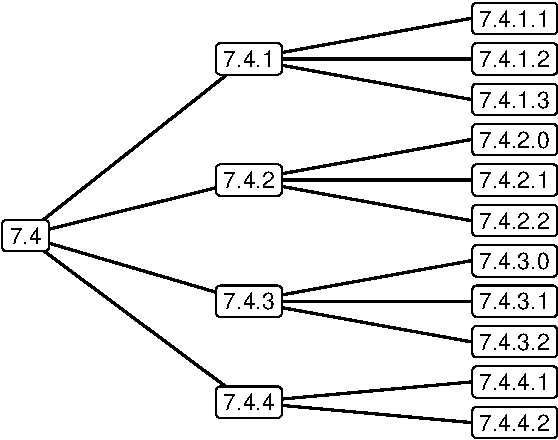
\includegraphics{moretrees_files/figure-latex/tree-1} \end{center}

Next, we load the data, check that the unique values in
\texttt{outcomes} are the same as the leaves of the tree
(\texttt{moretrees()} will throw an error if the latter isn't true, but
it's good practice to double-check before hand), and print the number of
matched pairs per outcome.

\begin{Shaded}
\begin{Highlighting}[]
\KeywordTok{data}\NormalTok{(}\StringTok{"moretreesExampleData"}\NormalTok{)}
\NormalTok{Xcase <-}\StringTok{ }\NormalTok{moretreesExampleData}\OperatorTok{$}\NormalTok{Xcase}
\NormalTok{Xcontrol <-}\StringTok{ }\NormalTok{moretreesExampleData}\OperatorTok{$}\NormalTok{Xcontrol}
\NormalTok{Wcase <-}\StringTok{ }\NormalTok{moretreesExampleData}\OperatorTok{$}\NormalTok{Wcase}
\NormalTok{Wcontrol <-}\StringTok{ }\NormalTok{moretreesExampleData}\OperatorTok{$}\NormalTok{Wcontrol}
\NormalTok{outcomes <-}\StringTok{ }\NormalTok{moretreesExampleData}\OperatorTok{$}\NormalTok{outcomes}
\NormalTok{leaves <-}\StringTok{ }\KeywordTok{names}\NormalTok{(}\KeywordTok{V}\NormalTok{(tr)[}\KeywordTok{degree}\NormalTok{(tr, }\DataTypeTok{mode =} \StringTok{"out"}\NormalTok{) }\OperatorTok{==}\StringTok{ }\DecValTok{0}\NormalTok{])}
\KeywordTok{setequal}\NormalTok{(leaves, }\KeywordTok{unique}\NormalTok{(outcomes))}
\CommentTok{#> [1] TRUE}
\NormalTok{knitr}\OperatorTok{::}\KeywordTok{kable}\NormalTok{(}\KeywordTok{table}\NormalTok{(outcomes))}
\end{Highlighting}
\end{Shaded}

\begin{longtable}[]{@{}lr@{}}
\toprule
outcomes & Freq\tabularnewline
\midrule
\endhead
7.4.1.1 & 80\tabularnewline
7.4.1.2 & 89\tabularnewline
7.4.1.3 & 98\tabularnewline
7.4.2.0 & 72\tabularnewline
7.4.2.1 & 68\tabularnewline
7.4.2.2 & 118\tabularnewline
7.4.3.0 & 97\tabularnewline
7.4.3.1 & 91\tabularnewline
7.4.3.2 & 97\tabularnewline
7.4.4.1 & 89\tabularnewline
7.4.4.2 & 101\tabularnewline
\bottomrule
\end{longtable}

We see that there are between 68 and 118 matched pairs per outcome. Note
that each case is associated with \emph{exactly one} outcome; the model
assumes cases do not experience multiple outcomes.

\hypertarget{model-without-covariate-adjustment}{%
\subsection{Model without covariate
adjustment}\label{model-without-covariate-adjustment}}

We now fit the MOReTreeS model without adjustment for covariates.

\begin{Shaded}
\begin{Highlighting}[]
\NormalTok{mod1 <-}\StringTok{ }\NormalTok{moretrees}\OperatorTok{::}\KeywordTok{moretrees}\NormalTok{(}\DataTypeTok{Xcase =}\NormalTok{ Xcase, }\DataTypeTok{Xcontrol =}\NormalTok{ Xcontrol,}
                 \DataTypeTok{outcomes =}\NormalTok{ outcomes, }\DataTypeTok{tr =}\NormalTok{ tr,}
                 \DataTypeTok{nrestarts =} \DecValTok{1}\NormalTok{, }\DataTypeTok{print_freq =} \DecValTok{500}\NormalTok{)}
\CommentTok{#> }
\CommentTok{#> Initialising restart 1 ...}
\CommentTok{#> }
\CommentTok{#> Iteration 500 ; epsilon = 0.00619 }
\CommentTok{#> Iteration 1000 ; epsilon = 0.00153876 }
\CommentTok{#> Iteration 1500 ; epsilon = 0.0003929994 }
\CommentTok{#> Iteration 2000 ; epsilon = 0.0001030746 }
\CommentTok{#> }
\CommentTok{#> Restart 1 complete.}
\end{Highlighting}
\end{Shaded}

We see that the model ran for at least 2000 iterations before converging
at a tolerance of \texttt{tol\ =\ 1E-8} (the default). The option
\texttt{print\_freq} determines how frequently the algorithm's progress
will be printed.

We now print the estimated odds ratios (or rate ratios, for a
case-crossover model) for the groups discovered by MOReTreeS. The table
also shows which outcomes belong to each group and the number of
observations associated with outcomes in each group.

\begin{Shaded}
\begin{Highlighting}[]
\KeywordTok{print}\NormalTok{(mod1, }\DataTypeTok{digits =} \DecValTok{2}\NormalTok{)}
\CommentTok{#> Group-specific exposure effect estimates for the 6 groups discovered by MOReTreeS}
\CommentTok{#> ------------------ Group 1 ------------------}
\CommentTok{#> }
\CommentTok{#> Number of outcomes: 3 }
\CommentTok{#> Number of matched pairs: 267 }
\CommentTok{#> List of outcomes:}
\CommentTok{#> 7.4.1.1, 7.4.1.2, 7.4.1.3 }
\CommentTok{#> }
\CommentTok{#> Odds ratio estimate(s):}
\CommentTok{#> }
\CommentTok{#>        dim    est    cil    ciu}
\CommentTok{#> ----  ----  -----  -----  -----}
\CommentTok{#> 1.1      1   1.68   1.37   2.05}
\CommentTok{#> 1.2      2   1.86   1.51   2.30}
\CommentTok{#> }
\CommentTok{#> ------------------ Group 2 ------------------}
\CommentTok{#> }
\CommentTok{#> Number of outcomes: 2 }
\CommentTok{#> Number of matched pairs: 190 }
\CommentTok{#> List of outcomes:}
\CommentTok{#> 7.4.4.1, 7.4.4.2 }
\CommentTok{#> }
\CommentTok{#> Odds ratio estimate(s):}
\CommentTok{#> }
\CommentTok{#>        dim    est    cil    ciu}
\CommentTok{#> ----  ----  -----  -----  -----}
\CommentTok{#> 1.1      1   1.78   1.41   2.25}
\CommentTok{#> 1.2      2   2.20   1.72   2.80}
\CommentTok{#> }
\CommentTok{#> ------------------ Group 3 ------------------}
\CommentTok{#> }
\CommentTok{#> Number of outcomes: 1 }
\CommentTok{#> Number of matched pairs: 97 }
\CommentTok{#> List of outcomes:}
\CommentTok{#> 7.4.3.0 }
\CommentTok{#> }
\CommentTok{#> Odds ratio estimate(s):}
\CommentTok{#> }
\CommentTok{#>        dim    est    cil    ciu}
\CommentTok{#> ----  ----  -----  -----  -----}
\CommentTok{#> 1.1      1   2.83   1.88   4.24}
\CommentTok{#> 1.2      2   1.02   0.71   1.47}
\CommentTok{#> }
\CommentTok{#> ------------------ Group 4 ------------------}
\CommentTok{#> }
\CommentTok{#> Number of outcomes: 2 }
\CommentTok{#> Number of matched pairs: 188 }
\CommentTok{#> List of outcomes:}
\CommentTok{#> 7.4.3.1, 7.4.3.2 }
\CommentTok{#> }
\CommentTok{#> Odds ratio estimate(s):}
\CommentTok{#> }
\CommentTok{#>        dim    est    cil    ciu}
\CommentTok{#> ----  ----  -----  -----  -----}
\CommentTok{#> 1.1      1   5.14   4.07   6.49}
\CommentTok{#> 1.2      2   2.48   2.01   3.06}
\CommentTok{#> }
\CommentTok{#> ------------------ Group 5 ------------------}
\CommentTok{#> }
\CommentTok{#> Number of outcomes: 3 }
\CommentTok{#> Number of matched pairs: 258 }
\CommentTok{#> List of outcomes:}
\CommentTok{#> 7.4.2.0, 7.4.2.1, 7.4.2.2 }
\CommentTok{#> }
\CommentTok{#> Odds ratio estimate(s):}
\CommentTok{#> }
\CommentTok{#>        dim    est    cil    ciu}
\CommentTok{#> ----  ----  -----  -----  -----}
\CommentTok{#> 1.1      1   6.33   4.89   8.20}
\CommentTok{#> 1.2      2   0.80   0.65   0.99}
\CommentTok{#> }
\CommentTok{#> }
\CommentTok{#> If this is hard to read, try print(x, compact = TRUE)}
\end{Highlighting}
\end{Shaded}

We can also plot the discovered groups on the outcome tree:

\begin{Shaded}
\begin{Highlighting}[]
\KeywordTok{plot}\NormalTok{(mod1, }\DataTypeTok{layout =} \StringTok{"slanted"}\NormalTok{, }\DataTypeTok{horizontal =} \OtherTok{FALSE}\NormalTok{)}
\end{Highlighting}
\end{Shaded}

\begin{center}\includegraphics{moretrees_files/figure-latex/tree_est-1} \end{center}

Finally, for comparison, we inspect the group-specific estimates
obtained by running a classical CLR model on the data for each
discovered group separately. Here, we use a more compact printing method
to save space.

\begin{Shaded}
\begin{Highlighting}[]
\KeywordTok{print}\NormalTok{(mod1, }\DataTypeTok{compact =}\NormalTok{ T, }\DataTypeTok{digits =} \DecValTok{2}\NormalTok{, }
      \DataTypeTok{coeff_type =} \StringTok{"clr"}\NormalTok{, }\DataTypeTok{print_outcomes =} \OtherTok{FALSE}\NormalTok{)}
\CommentTok{#> Showing conditional logistic regression estimates for discovered groups.}
\CommentTok{#> }
\CommentTok{#> Group-specific odds ratio estimate(s):}
\CommentTok{#> }
\CommentTok{#>  group   n_outcomes   n_obs   est1   cil1    ciu1   est2   cil2   ciu2}
\CommentTok{#> ------  -----------  ------  -----  -----  ------  -----  -----  -----}
\CommentTok{#>      1            3     267   1.65   1.36    2.03   1.86   1.50   2.35}
\CommentTok{#>      2            2     190   1.76   1.39    2.28   2.21   1.69   2.99}
\CommentTok{#>      3            1      97   2.62   1.76    4.21   0.98   0.71   1.35}
\CommentTok{#>      4            2     188   6.99   4.11   13.36   3.00   2.07   4.69}
\CommentTok{#>      5            3     258   7.26   4.62   12.43   0.77   0.61   0.97}
\end{Highlighting}
\end{Shaded}

\hypertarget{model-with-covariate-adjustment}{%
\subsection{Model with covariate
adjustment}\label{model-with-covariate-adjustment}}

Next, we fit the MOReTreeS model \emph{with} covariate adjustment. For
parameters that were estimated in the model \emph{without} covariate
adjustment, we use the final model values as initial values in the
adjusted model. This approach may be useful for speeding up models with
covariates, which can be slower to converge than unadjusted models.

\begin{Shaded}
\begin{Highlighting}[]
\NormalTok{vi_params_init <-}\StringTok{ }\NormalTok{mod1}\OperatorTok{$}\NormalTok{mod}\OperatorTok{$}\NormalTok{vi_params[}\KeywordTok{c}\NormalTok{(}\StringTok{"prob"}\NormalTok{, }\StringTok{"mu"}\NormalTok{, }\StringTok{"Sigma"}\NormalTok{,}
                                       \StringTok{"Sigma_inv"}\NormalTok{, }\StringTok{"Sigma_det"}\NormalTok{,}
                                       \StringTok{"tau_t"}\NormalTok{, }\StringTok{"a_t"}\NormalTok{, }\StringTok{"b_t"}\NormalTok{)]}
\NormalTok{hyperparams_init <-}\StringTok{ }\NormalTok{mod1}\OperatorTok{$}\NormalTok{mod}\OperatorTok{$}\NormalTok{hyperparams[}\KeywordTok{c}\NormalTok{(}\StringTok{"eta"}\NormalTok{, }\StringTok{"tau"}\NormalTok{)]}
\NormalTok{mod2 <-}\StringTok{ }\NormalTok{moretrees}\OperatorTok{::}\KeywordTok{moretrees}\NormalTok{(}\DataTypeTok{Xcase =}\NormalTok{ Xcase, }\DataTypeTok{Xcontrol =}\NormalTok{ Xcontrol,}
                  \DataTypeTok{Wcase =}\NormalTok{ Wcase, }\DataTypeTok{Wcontrol =}\NormalTok{ Wcontrol,}
                  \DataTypeTok{vi_params_init =}\NormalTok{ vi_params_init,}
                  \DataTypeTok{hyperparams_init =}\NormalTok{ hyperparams_init,}
                  \DataTypeTok{outcomes =}\NormalTok{ outcomes, }\DataTypeTok{tr =}\NormalTok{ tr,}
                  \DataTypeTok{nrestarts =} \DecValTok{1}\NormalTok{, }\DataTypeTok{print_freq =} \DecValTok{1000}\NormalTok{)}
\CommentTok{#> }
\CommentTok{#> Initialising restart 1 ...}
\CommentTok{#> }
\CommentTok{#> Iteration 1000 ; epsilon = 0.008971813 }
\CommentTok{#> Iteration 2000 ; epsilon = 0.00192693 }
\CommentTok{#> Iteration 3000 ; epsilon = 0.000806864 }
\CommentTok{#> Iteration 4000 ; epsilon = 0.0004397234 }
\CommentTok{#> Iteration 5000 ; epsilon = 0.0002758774 }
\CommentTok{#> Iteration 5000 complete.}
\CommentTok{#> Warning in spike_and_slab_logistic_moretrees(dsgn = dsgn, vi_params_init =}
\CommentTok{#> vi_params_init, : Maximum number of iterations reached! Consider increasing}
\CommentTok{#> max_iter.}
\CommentTok{#> }
\CommentTok{#> Restart 1 complete.}
\end{Highlighting}
\end{Shaded}

The warning indicates that the default maximum number of iterations,
\texttt{max\_iter\ =\ 5000}, was reached before the model converged. We
therefore increase \texttt{max\_iter} and run the model again, using as
new starting values the final values from the run which failed to
converge.

\begin{Shaded}
\begin{Highlighting}[]
\NormalTok{vi_params_init <-}\StringTok{ }\NormalTok{mod2}\OperatorTok{$}\NormalTok{mod}\OperatorTok{$}\NormalTok{vi_params}
\NormalTok{hyperparams_init <-}\StringTok{ }\NormalTok{mod2}\OperatorTok{$}\NormalTok{mod}\OperatorTok{$}\NormalTok{hyperparams}
\NormalTok{mod2 <-}\StringTok{ }\NormalTok{moretrees}\OperatorTok{::}\KeywordTok{moretrees}\NormalTok{(}\DataTypeTok{Xcase =}\NormalTok{ Xcase, }\DataTypeTok{Xcontrol =}\NormalTok{ Xcontrol,}
                  \DataTypeTok{Wcase =}\NormalTok{ Wcase, }\DataTypeTok{Wcontrol =}\NormalTok{ Wcontrol,}
                  \DataTypeTok{vi_params_init =}\NormalTok{ vi_params_init,}
                  \DataTypeTok{hyperparams_init =}\NormalTok{ hyperparams_init,}
                  \DataTypeTok{outcomes =}\NormalTok{ outcomes, }\DataTypeTok{tr =}\NormalTok{ tr,}
                  \DataTypeTok{nrestarts =} \DecValTok{1}\NormalTok{, }\DataTypeTok{print_freq =} \DecValTok{1000}\NormalTok{,}
                  \DataTypeTok{max_iter =} \DecValTok{10000}\NormalTok{)}
\CommentTok{#> }
\CommentTok{#> Initialising restart 1 ...}
\CommentTok{#> }
\CommentTok{#> Iteration 1000 ; epsilon = 0.0001889536 }
\CommentTok{#> Iteration 2000 ; epsilon = 0.0001374139 }
\CommentTok{#> Iteration 3000 ; epsilon = 0.0001043828 }
\CommentTok{#> Iteration 4000 ; epsilon = 8.195984e-05 }
\CommentTok{#> Iteration 5000 ; epsilon = 6.604833e-05 }
\CommentTok{#> Iteration 6000 ; epsilon = 5.43529e-05 }
\CommentTok{#> }
\CommentTok{#> Restart 1 complete.}
\end{Highlighting}
\end{Shaded}

The model has now converged. Next, we print the estimated odds ratios
for the discovered groups \emph{adjusted for the covariates in}
\texttt{W}. We suppress printing of the outcomes associated with each
group, since in this example these happen to be the same as for the
model with no covariates.

\begin{Shaded}
\begin{Highlighting}[]
\KeywordTok{print}\NormalTok{(mod2, }\DataTypeTok{compact =}\NormalTok{ T, }\DataTypeTok{digits =} \DecValTok{2}\NormalTok{, }\DataTypeTok{print_outcomes =} \OtherTok{FALSE}\NormalTok{)}
\CommentTok{#> Group-specific odds ratio estimate(s):}
\CommentTok{#> }
\CommentTok{#>  group   n_outcomes   n_obs   est1   cil1   ciu1   est2   cil2   ciu2}
\CommentTok{#> ------  -----------  ------  -----  -----  -----  -----  -----  -----}
\CommentTok{#>      1            3     267   1.74   1.42   2.14   2.01   1.62   2.50}
\CommentTok{#>      2            2     190   1.88   1.48   2.38   2.19   1.71   2.80}
\CommentTok{#>      3            1      97   3.07   2.02   4.68   1.10   0.76   1.59}
\CommentTok{#>      4            2     188   5.74   4.51   7.29   2.94   2.37   3.64}
\CommentTok{#>      5            3     258   7.27   5.58   9.48   0.80   0.65   0.99}
\end{Highlighting}
\end{Shaded}

\hypertarget{using-random-restarts}{%
\subsection{Using random restarts}\label{using-random-restarts}}

Note that in the example above, we have used only
\texttt{nrestarts\ =\ 1} random restarts for illustration purposes. This
means we have chosen only one non-random set of initial values for the
VI algorithm. However, in practice we recommend using
\texttt{nrestarts\ \textgreater{}\ 1}. This will cause
\texttt{moretrees()} to run multiple versions of the VI algorithm from
different random initial values. These restarts may converge to
different local optima; if so, the ``best'' restart will be returned
(highest value of the objective function). Here, we use the initial
values from \texttt{mod2} with some randomness added for each restart.

The unevaluated code chunk below illustrates how to register a parallel
backend for running three random restarts on three cores. When
\texttt{nrestarts\ \textgreater{}\ 1}, \texttt{moretrees()} attempts to
run the restarts on multiple cores by default. To prevent this behaviour
and run the restarts on one core, use the option
\texttt{parallel\ =\ FALSE}. The progress of restart \texttt{i} will be
logged to a text file \texttt{restart\_logs/restart\_i\_log.txt} which
is deleted at the end of the run. \texttt{moretrees} returns the results
from the `best' restart, and by default stores the results from the
other restarts in the list item \texttt{mod\_restarts}. For large
models, preserving the restarts can lead to memory problems; these can
be discarded using the option \texttt{keep\_restarts\ =\ FALSE}.

\begin{Shaded}
\begin{Highlighting}[]
\NormalTok{nrestarts <-}\StringTok{ }\DecValTok{3}
\NormalTok{doParallel}\OperatorTok{::}\KeywordTok{registerDoParallel}\NormalTok{(}\DataTypeTok{cores =}\NormalTok{ nrestarts)}
\KeywordTok{set.seed}\NormalTok{(}\DecValTok{345083}\NormalTok{)}
\NormalTok{log_dir <-}\StringTok{ "restart_logs"}
\KeywordTok{dir.create}\NormalTok{(log_dir)}
\NormalTok{mod3 <-}\StringTok{ }\NormalTok{moretrees}\OperatorTok{::}\KeywordTok{moretrees}\NormalTok{(}\DataTypeTok{Xcase =}\NormalTok{ Xcase, }\DataTypeTok{Xcontrol =}\NormalTok{ Xcontrol,}
                  \DataTypeTok{Wcase =}\NormalTok{ Wcase, }\DataTypeTok{Wcontrol =}\NormalTok{ Wcontrol,}
                  \DataTypeTok{outcomes =}\NormalTok{ outcomes, }\DataTypeTok{tr =}\NormalTok{ tr,}
                  \DataTypeTok{vi_params_init =}\NormalTok{ mod2}\OperatorTok{$}\NormalTok{mod}\OperatorTok{$}\NormalTok{vi_params,}
                  \DataTypeTok{hyperparams_init =}\NormalTok{ mod2}\OperatorTok{$}\NormalTok{mod}\OperatorTok{$}\NormalTok{hyperparams,}
                  \DataTypeTok{nrestarts =}\NormalTok{ nrestarts, }\DataTypeTok{print_freq =} \DecValTok{500}\NormalTok{,}
                  \DataTypeTok{log_restarts =} \OtherTok{TRUE}\NormalTok{, }\DataTypeTok{log_dir =}\NormalTok{ log_dir)}
\KeywordTok{unlink}\NormalTok{(log_dir, }\DataTypeTok{recursive =}\NormalTok{ T)}
\CommentTok{# Print the final ELBO for all restarts}
\KeywordTok{print}\NormalTok{(}\KeywordTok{c}\NormalTok{(mod3}\OperatorTok{$}\NormalTok{mod}\OperatorTok{$}\NormalTok{hyperparams}\OperatorTok{$}\NormalTok{ELBO,}
  \KeywordTok{sapply}\NormalTok{(mod3}\OperatorTok{$}\NormalTok{mod_restarts, }\ControlFlowTok{function}\NormalTok{(mod) mod}\OperatorTok{$}\NormalTok{hyperparams}\OperatorTok{$}\NormalTok{ELBO)),}
  \DataTypeTok{digits =} \DecValTok{8}\NormalTok{)}
\end{Highlighting}
\end{Shaded}

\hypertarget{algo}{%
\section{Details of variational inference algorithm}\label{algo}}

VI is a method for approximating the posterior distribution of a
Bayesian model. This is achieved by minimizing the ``distance'' between
a pre-specified family of probability distributions \(q\) and the true
posterior \(\pi\), where distance is typically defined as the
Kullback-Leibler divergence \(K(q || \pi)\). Using this technique, VI
finds a \emph{deterministic} approximation for \(\pi\), in contrast to
MCMC which attempts to sample from \(\pi\). A detailed introduction to
VI is beyond the scope of this vignette; for an accessible introduction
for statisticians, see Blei, Kucukelbir, and McAuliffe (2017).

This section of the vignette is \emph{not} required reading. Rather, it
is intended for readers with some knowledge of variational Bayes who may
wish to verify the details of the VI algorithm used by
\texttt{moretrees}.

\hypertarget{preliminaries}{%
\subsection{Preliminaries}\label{preliminaries}}

We take a mean field VI apprach and assume that the variational
approximation \(q\) factorizes as
\(q\left(\boldsymbol{\gamma},\mathbf{s}, \boldsymbol{\theta}, \boldsymbol{\rho} \right) = \prod_{u \in \mathcal{V}} q \left( \boldsymbol{\theta}_u \right) q\left(\boldsymbol{\gamma}_u, s_u \right) \prod_{l=1}^L q(\rho_l)\),
where \(\boldsymbol{\gamma}\), \(\mathbf{s}\), \(\boldsymbol{\theta}\),
and \(\boldsymbol{\rho}\) are vectors containing all
\(\boldsymbol{\gamma}_u\), \(\mathbf{s}_u\), \(\boldsymbol{\theta}_u\)
and \(\boldsymbol{\rho}_l\) respectively. Rather than minimizing
\(K(q || \pi)\), which depends on the intractable posterior \(\pi\), we
maximize a quantity known as the evidence lower bound (ELBO),
\(\mathcal{E}(q)\), which is equal to \(- K(q || \pi)\) up to an
additive constant that does not depend on \(q\):

\begin{equation}
\tag{2}
\mathcal{E}(q) = E_{q} \left[\log f \left(\boldsymbol{\gamma}, \mathbf{s}, \boldsymbol{\theta}, \boldsymbol{\rho} \right) \right] - E_{q} \left[\log q \left(\boldsymbol{\gamma}, \mathbf{s}, \boldsymbol{\theta}, \boldsymbol{\rho} \right) \right] 
\end{equation} where
\(f \left(\boldsymbol{\gamma}, \mathbf{s}, \boldsymbol{\theta}, \boldsymbol{\rho} \right)\)
is the joint density of data and parameters, and \(E_q\) denotes
expectation taken with respect to \(q\).

The \texttt{moretrees} packages uses a co-ordinate ascent variational
inference (CAVI) algorithm to maximize \(\mathcal{E}(q)\) in \(q\).
However, attempting to maximize \(\mathcal{E}(q)\) directly would lead
to intractable updates due to the logistic form of the likelihood in
Equation 1. We therefore replace this likelihood in the expression for
\(\mathcal{E}(q)\) with a quadratic approximation that leads to
tractable updates in the CAVI algorithm. This approach to VI with a
logistic likelihood was first proposed by Jaakkola and Jordan (2000).
Here, we state the result; see Bishop (2016 Section 10.6) for a detailed
derivation.

First, the joint density of data and parameters is:

\begin{align*}
f \left(\boldsymbol{\gamma}, \mathbf{s}, \boldsymbol{\theta}, \boldsymbol{\rho} \right) 
& = \prod_{v \in \mathcal{V}_l} \prod_{i = 1}^{n_v} \left(1 + \exp \left[-\left(\sum_{u \in a(v)} s_u \boldsymbol{\gamma}_u^T \mathbf{x}_{i}^{(u)} + \boldsymbol{\theta}_u^T \mathbf{w}_i^{(u)} \right) \right] \right)^{-1} \\
& \times \prod_{u \in \mathcal{V}} \rho_{l_u}^{s_u} (1-\rho_{l_u})^{1-s_u} \dfrac{1}{\left(2\pi\tau_{l_u}\right)^{k/2}} \exp\left[-\dfrac{\boldsymbol{\gamma}_u^T\boldsymbol{\gamma}_u}{2\tau_{l_u}}\right] \\
& \times \prod_{u \in \mathcal{V}} \dfrac{1}{\left(2\pi\omega_{l_u}\right)^{m/2}} \exp\left[-\dfrac{\boldsymbol{\theta}_u^T\boldsymbol{\theta}_u}{2\omega_{l_u}}\right] \\
& \times \prod_{l=1}^L \dfrac{\rho_l^{a_l -1} (1 - \rho_l)^{b_l - 1}}{\mathcal{B}(a_l, b_l)}.
\end{align*}

Next, let

\[r_i^{(v)} = \sum_{u \in a(v)} s_u \boldsymbol{\gamma}_u^T \mathbf{x}_{i}^{(u)} + \boldsymbol{\theta}_u^T \mathbf{w}_i^{(u)}.\]

Then a lower bound for the likelihood contribution from a single matched
pair is (Jaakkola and Jordan 2000): \begin{align*}
     \left(1 + \exp(-r_i^{(v)}) \right)^{-1}
    & \geq \sigma(\eta_i^{(v)}) \exp \left[ r_i^{(v)} - \left(r_i^{(v)} + \eta_i^{(v)} \right) /2 -g(\eta_i^{(v)}) \left[r_i^{(v)2} - \eta_i^{(v)2} \right] \right] \\
    & := h\left(\eta_i^{(v)}, r_i^{(v)} \right).
\end{align*}

where \(\sigma(x) = (1 + e^{-x})^{-1}\) and
\(g(x) = \dfrac{1}{2x}(\sigma(x) - 1/2)\). This inequality hold for all
values of \(\eta_i^{(v)}\), an introduced variational parameter.

Let
\(h\left(\boldsymbol{\eta}, \boldsymbol{\gamma}, \mathbf{s}, \boldsymbol{\theta}, \boldsymbol{\rho} \right) = \prod_{v \in \mathcal{V}_L} \prod_{i=1}^{n_v} h\left(\eta_i^{(v)}, r_i^{(v)} \right)\).
We get the following approximation to the joint density of data and
parameters:

\begin{equation*}
f \left(\boldsymbol{\gamma}, \mathbf{s}, \boldsymbol{\theta}, \boldsymbol{\rho} \right) \geq h\left(\boldsymbol{\eta}, \boldsymbol{\gamma}, \mathbf{s}, \boldsymbol{\theta}, \boldsymbol{\rho} \right) \pi \left(\boldsymbol{\gamma}, \mathbf{s}, \boldsymbol{\theta}, \boldsymbol{\rho} \right)
\end{equation*}

where
\(\pi \left(\boldsymbol{\gamma}, \mathbf{s}, \boldsymbol{\theta}, \boldsymbol{\rho} \right)\)
is the prior. We ensure this lower bound is as tight as possible by
maximizing it in \(\boldsymbol{\eta}\) at every step.

Replacing the joint density of data and parameters in Equation 2 with
the above lower bound gives the following approximation to the ELBO:

\begin{align*}
\mathcal{E}^*(q) & :=  E_{q} \left[\log h\left(\boldsymbol{\eta}, \boldsymbol{\gamma}, \mathbf{s}, \boldsymbol{\theta}, \boldsymbol{\rho} \right) \pi \left(\boldsymbol{\gamma}, \mathbf{s}, \boldsymbol{\theta}, \boldsymbol{\rho} \right) \right] - E_{q} \left[\log q \left(\boldsymbol{\gamma}, \mathbf{s}, \boldsymbol{\theta}, \boldsymbol{\rho} \right) \right] \leq \mathcal{E}(q).
\end{align*}

\hypertarget{co-ordinate-ascent-variational-inference-algorithm}{%
\subsection{Co-ordinate ascent variational inference
algorithm}\label{co-ordinate-ascent-variational-inference-algorithm}}

The CAVI algorithm involves maximizing \(\mathcal{E}^*(q)\) in each of
the factors \(q\left(\boldsymbol{\gamma}_u, s_u \right)\),
\(q \left( \boldsymbol{\theta}_u \right)\), and \(q(\rho_l)\) in turn.
In what follows we use the subscript \(t\) or superscript \((t)\) to
denote the next iteration or update in the CAVI algorithm; the absence
of a subscript indicates that the last or most recent value of that
parameter should be used.

The updates for each factor in the CAVI algorithm can be obtained using
the following well-known result (see Blei 2017 for a derivation). As an
example, consider the factor
\(q\left(\boldsymbol{\gamma}_u, s_u \right)\). Let
\(q_{-\left(\boldsymbol{\gamma}_u, s_u \right)}\) be the variational
distribution marginalized over \((\boldsymbol{\gamma}_u, s_u)\). Then
the \(t^{th}\) coordinate ascent update for
\(q(\boldsymbol{\gamma}_u, s_u)\) is given by:

\[ q_t \left( \boldsymbol{\gamma}_u, s_u \right) \propto \exp \left( E_{q_{-\left(\boldsymbol{\gamma}_u, s_u \right)}} \left[ \log f \left(\boldsymbol{\gamma}, \mathbf{s}, \boldsymbol{\theta}, \boldsymbol{\rho} \right) \right] \right).\]
However, here replace the joint density \(f\) with its quadratic
approximation to get

\[q_t \left( \boldsymbol{\gamma}_u, s_u \right) \propto \exp \left( E_{q_{-\left(\boldsymbol{\gamma}_u, s_u \right)}} \left[ \log h\left(\boldsymbol{\eta}, \boldsymbol{\gamma}, \mathbf{s}, \boldsymbol{\theta}, \boldsymbol{\rho} \right) \pi \left(\boldsymbol{\gamma}, \mathbf{s}, \boldsymbol{\theta}, \boldsymbol{\rho} \right) \right] \right).\]

The equivalent results hold for all other factors \(q(\rho_l)\),
\(q(\boldsymbol{\theta}_u)\), and \(q(\boldsymbol{\gamma}_v, s_v)\) for
\(v \neq u\).

Below, we give the CAVI updates for each factor. These updates can be
straightforwardly derived from the above formula. In the
\texttt{moretrees} package, these updates are coded in the internal
function \texttt{update\_vi\_params\_logistic\_moretrees()}.

\hypertarget{update-for-qboldsymbolgamma_u-s_u}{%
\subsubsection{\texorpdfstring{Update for
\(q(\boldsymbol{\gamma}_u, s_u)\)}{Update for q(\textbackslash{}boldsymbol\{\textbackslash{}gamma\}\_u, s\_u)}}\label{update-for-qboldsymbolgamma_u-s_u}}

\[ q_{t}\left( \boldsymbol{\gamma}_u, s_u \right) = \mathcal{MVN}\left(\boldsymbol{\gamma}_u \middle\vert s_u \boldsymbol{\mu}_u^{(t)}, s_u \Sigma_u^{(t)} + (1-s_u) \tilde{\tau}_u^{(t)} I_{k} \right) p_u^{(t)s_u} \left(1-p_u^{(t)}\right)^{1-s_u}\]

where

\begin{align*}
\left(\Sigma_u^{(t)}\right)^{-1} & = \dfrac{1}{\tau_{l_u}} I_{k} + 2 \sum_{v: u \in anc(v)} \eta_i^{(v)} \mathbf{x}_i^{(v)} \mathbf{x}_i^{(v)T} \\
\tilde{\tau}_u^{(t)} & = \tau_{l_u} \\
\boldsymbol{\mu}_u^{(t)} & =  \Sigma_u^{(t)} \sum_{v: u \in anc(v)} \sum_{i = 1}^{n_v} \mathbf{x}_i^{(v)} \left(\dfrac{1}{2} - 2 g \left(\eta_i^{(v)}\right)\left( \sum_{u^\prime \in anc(v)} E_{q} \left[ \boldsymbol{\theta}_{u^\prime} \right]^T \mathbf{w}_i^{(v)} +   \sum_{u^\prime \in anc(v) \backslash \lbrace u \rbrace} E_{q}  \left[ \boldsymbol{\gamma}_{u^\prime} s_{u^\prime} \right]^T \mathbf{x}_i^{(v)} \right) \right) \\
\log \left(\dfrac{p_u^{(t)}}{ 1- p_u^{(t)}} \right) & =  E_{q} \left[ \log \rho_{l_u} \right] - E_{q} \left[ \log (1-\rho_{l_u})\right] + \dfrac{\boldsymbol{\mu}_u^{(t)T} \left(\Sigma_u^{(t)}\right)^{-1} \boldsymbol{\mu}_u^{(t)}}{2} + \dfrac{1}{2} \left( \log \left\vert \Sigma_u^{(t)} \right\vert - k \log \tilde{\tau}_u^{(t)} \right).
\end{align*}

\hypertarget{update-for-qboldsymboltheta_u}{%
\subsubsection{\texorpdfstring{Update for
\(q(\boldsymbol{\theta}_u)\)}{Update for q(\textbackslash{}boldsymbol\{\textbackslash{}theta\}\_u)}}\label{update-for-qboldsymboltheta_u}}

\[q_t\left( \boldsymbol{\theta}_u \right) = \mathcal{MVN}\left(\boldsymbol{\delta}_u, \Omega_u \right) \]
where

\begin{align*}
\left(\Omega_u^{(t)}\right)^{-1} & = \dfrac{1}{\omega_{l_u}} I_m + 2 \sum_{v: u \in anc(v)} \sum_{i=1}^{n_v} g(\eta_i^{(v)}) \mathbf{w}_i^{(v)} \mathbf{w}_i^{(v)T}  \\
\boldsymbol{\delta}_u^{(t)} & =  \Omega_u^{(t)} \sum_{v: u \in anc(v)} \sum_{i=1}^{n_v} \mathbf{w}_i^{(v)} \left( \dfrac{1}{2} - 2 g\left(\eta_i^{(v)}\right) \left( \sum_{u^\prime \in anc(v) \backslash \lbrace u \rbrace} E_{q} \left[ \boldsymbol{\theta}_{u^\prime} \right]^T \mathbf{w}_i^{(v)} +   \sum_{u^\prime \in anc(v) \rbrace} E_{q}  \left[ \boldsymbol{\gamma}_{u^\prime} s_{u^\prime} \right]^T \mathbf{x}_i^{(v)} \right) \right).
\end{align*}

\hypertarget{update-for-qrho_l}{%
\subsubsection{\texorpdfstring{Update for
\(q(\rho_l)\)}{Update for q(\textbackslash{}rho\_l)}}\label{update-for-qrho_l}}

\[q_{t}(\rho_l) = Beta \left(\tilde{a}_l^{(t)}, \tilde{b}_l^{(t)} \right)\]

where

\begin{align*}
\tilde{a}_l^{(t)} & = a_l + \sum_{u: l_u = l}  E_{q} \left[ s_u \right] \\
\tilde{b}_l^{(t)} & = b_l + \sum_{u: l_u = l}  E_{q} \left[ 1 - s_u \right].
\end{align*}

\hypertarget{objective-function-evidence-lower-bound}{%
\subsection{Objective function (evidence lower
bound)}\label{objective-function-evidence-lower-bound}}

At the end of every iteration \(t\) we must compute the objective
function \(\mathcal{E}^*(q_t)\) for the current value of our variational
approximation \(q_t\). We iterate through parameter updates until
convergence, i.e.,
\(\left\vert \mathcal{E}^*(q_t) - \mathcal{E}^*(q_{t-1}) \right\vert <\)
\texttt{tol}.

\begin{align}
\mathcal{E}^*(q) & =  \sum_{v \in \mathcal{V}_L} \sum_{i = 1}^{n_v} \left( \dfrac{1}{2}E_q \left[ r_i^{(v)} \right] + \log \sigma\left(\eta_i^{(v)}\right) - \eta_i^{(v)} / 2 + g\left(\eta_i^{(v)}\right) \left(\eta_i^{(v)2} - E_q \left[r_i^{(v)2} \right]  \right) \right) \tag{1} \\
& - \sum_{u \in \mathcal{V}}\left( \dfrac{E_q \left[\boldsymbol{\gamma}_u^T\boldsymbol{\gamma}_u \right]}{2\tau_{l_u}} + \dfrac{k}{2} \log(2 \pi \tau_{l_u})\right)  \tag{2} \\
& +  \sum_{u \in \mathcal{V}} E_q \left[ \log \rho_{l_u} \right]  E_q \left[ s_u \right]  + E \left[ \log \left(1 - \rho_{l_u} \right) \right] \left(1-E \left[s_u\right] \right)   \tag{3} \\
& - \sum_{u \in \mathcal{V}} \dfrac{E \left[\boldsymbol{\theta}_u^T \boldsymbol{\theta}_u \right]}{2 \omega_{l_u}} - \dfrac{m}{2} \log (2 \pi \omega_{l_u})  \tag{4} \\
& + \sum_{l = 1}^L \left((a_l - 1) E_q \left[\log \rho_l \right] + (b_l - 1) E_q \left[\log (1 - \rho_l) \right] - \log \mathcal{B} (a_l, b_l) \right)  \tag{5} \\
& + \dfrac{1}{2} \sum_{u \in \mathcal{V}} E_q\left[s_u \left(\boldsymbol{\gamma}_u - \boldsymbol{\mu}_u \right)^T \Sigma_u^{-1} \left(\boldsymbol{\gamma}_u - \boldsymbol{\mu}_u \right) \right] + \dfrac{1}{2} E_q\left[ s_u \right] \left( \log \left\vert \Sigma_u \right\vert + k \log (2\pi)\right)  \tag{6} \\
& + \dfrac{1}{2} \sum_{u \in \mathcal{V}} \dfrac{1}{\tilde{\tau}_u} E_q\left[(1-s_u) \boldsymbol{\gamma}_u^T \boldsymbol{\gamma}_u \right] +  \dfrac{k}{2} \log (2\pi \tilde{\tau}_u) E_q\left[ 1-s_u \right]  \tag{7} \\
& - \sum_{u \in \mathcal{V}} \left( E_q[s_u] \log(p_u) + E_q[1-s_u] \log \left( 1- p_u \right) \right)  \tag{8} \\ 
& + \dfrac{1}{2} \sum_{u \in \mathcal{V}} E_q \left[ \left(\boldsymbol{\theta}_u - \boldsymbol{\delta}_u \right)^T \Omega_u^{-1} \left(\boldsymbol{\theta}_u - \boldsymbol{\delta}_u \right) \right] +  \dfrac{1}{2} \log \left\vert \Omega_u \right\vert + \dfrac{m}{2} \log(2 \pi)  \tag{9} \\
& - \sum_{l = 1}^L \left((\tilde{a}_l - 1) E_q \left[\log \rho_l \right] + (\tilde{b}_l - 1) E \left[\log (1 - \rho_l) \right] - \log \mathcal{B} (\tilde{a}_l, \tilde{b}_l) \right).  \tag{10}
\end{align}

where \(\mathcal{B}(\cdot,\cdot)\) is the Beta function. The
expectations with respect to \(q\) can be computed using the known
expressions for each factor of \(q\) given in the previous sections
(recall that \(r_i^{(v)}\) depends on the parameters
\(\boldsymbol{\gamma}\), \(\mathbf{s}\), and \(\boldsymbol{\theta}\)).
The line numbers above correspond exactly to those used in the internal
function \texttt{update\_hyperparams\_logistic\_moretrees()}, which both
computes \(\mathcal{E}^*(q)\) and performs the hyperparameter updates
described in the next section.

\hypertarget{hyperparameter-selection}{%
\subsection{Hyperparameter selection}\label{hyperparameter-selection}}

The hyperparameters \(\tau_l\) and \(\omega_l\) for \(l = 1, \dots, L\)
are selected via approximate empirical Bayes. Specifically, every
\texttt{update\_hyper\_freq} iterations, we maximize
\(\mathcal{E}^*(q)\), which can be viewed as an approximation to the
marginal likelihood, in each hyperparameter. This gives the following
hyperparameter updates:

\begin{align*}
\tau_l^{(t)} & = \dfrac{\sum_{u: l_u = u} E_{q}\left[ \boldsymbol{\gamma}_u^T \boldsymbol{\gamma}_u \right]}{\sum_{u: l_u = u} k} \\
\omega_l^{(t)} & = \dfrac{\sum_{u: l_u = u} E_{q} \left[ \boldsymbol{\theta}_u^T \boldsymbol{\theta}_u \right]}{\sum_{u: l_u = u} m}.
\end{align*}

This convenient technique has been used elsewhere (Blei, Ng, and Jordan
2003; Khan et al. 2010). It is particularly useful in the case of
estimating the variance parameters \(\tau_l\) and \(\omega_l\), since in
the absence of prior information, specifying good non-informative priors
for variance parameters, such as those recommended by Gelman (2006),
would require breaking the conditional conjugacy that leads to
closed-form updates in the VI algorithm.

Ideally, one would find the optimal VI parameters after every
hyperparameter update by allowing the algorithm to converge while
keeping the hyperparameters fixed. The hyperparameters would then be
updated again, and this process would be repeated until convergence of
both the VI parameters and hyperparameters. However, in practice this
can be too time consuming; as an alternative, we set a maximum of
\texttt{update\_hyper\_freq} VI updates between hyperparameter updates.
The default value is \texttt{update\_hyper\_freq\ =\ 50}; if the
algorithm is converging slowly, either increasing or decreasing this
value may help.

We also allow a different convergence tolerance, \texttt{tol\_hyper},
when comparing \(\mathcal{E}^*(q)\) between consecutive hyperparameter
updates. The algorithm is considered to have converged when the
difference in \(\mathcal{E}^*(q)\) between consecutive hyperparameter
updates is less than \texttt{tol\_hyper} \emph{and} the difference
between the last two variational parameter updates is less than
\texttt{tol}. If our aim in selecting hyperparameters is merely to
identify `good enough' values, it may be acceptable to set
\texttt{tol\_hyper} \(<\) \texttt{tol}. Because convergence of the
hyperparameters can be slow, this also allows us to speed up convergence
of the algorithm overall.

\hypertarget{references}{%
\section*{References}\label{references}}
\addcontentsline{toc}{section}{References}

\hypertarget{refs}{}
\leavevmode\hypertarget{ref-barbieri2004optimal}{}%
Barbieri, Maria Maddalena, and James O Berger. 2004. ``Optimal
Predictive Model Selection.'' \emph{The Annals of Statistics} 32 (3).
Institute of Mathematical Statistics: 870--97.

\leavevmode\hypertarget{ref-bishop2016pattern}{}%
Bishop, Christopher M. 2016. \emph{Pattern Recognition and Machine
Learning}. Springer-Verlag New York.

\leavevmode\hypertarget{ref-blei2017variational}{}%
Blei, David M, Alp Kucukelbir, and Jon D McAuliffe. 2017. ``Variational
Inference: A Review for Statisticians.'' \emph{Journal of the American
Statistical Association} 112 (518). Taylor \& Francis: 859--77.

\leavevmode\hypertarget{ref-blei2003latent}{}%
Blei, David M, Andrew Y Ng, and Michael I Jordan. 2003. ``Latent
Dirichlet Allocation.'' \emph{Journal of Machine Learning Research} 3:
993--1022.

\leavevmode\hypertarget{ref-gelman2006prior}{}%
Gelman, Andrew. 2006. ``Prior Distributions for Variance Parameters in
Hierarchical Models.'' \emph{Bayesian Analysis} 1 (3). International
Society for Bayesian Analysis: 515--34.

\leavevmode\hypertarget{ref-healthcare2018clinical}{}%
Healthcare Cost and Utilization Project. 2018. ``Clinical
Classifications Software (CCS) for ICD-9-CM.''
\href{www.\%20hcup-us.ahrq.\%20gov/toolssoftware/ccs/ccs}{www. hcup-us.ahrq. gov/toolssoftware/ccs/ccs}.

\leavevmode\hypertarget{ref-jaakkola2000bayesian}{}%
Jaakkola, Tommi S, and Michael I Jordan. 2000. ``Bayesian Parameter
Estimation via Variational Methods.'' \emph{Statistics and Computing} 10
(1). Springer: 25--37.

\leavevmode\hypertarget{ref-khan2010variational}{}%
Khan, Mohammad E, Guillaume Bouchard, Kevin P Murphy, and Benjamin M
Marlin. 2010. ``Variational Bounds for Mixed-Data Factor Analysis.'' In
\emph{Advances in Neural Information Processing Systems}, 1108--16.

\leavevmode\hypertarget{ref-maclure1991case}{}%
Maclure, Malcolm. 1991. ``The Case-Crossover Design: A Method for
Studying Transient Effects on the Risk of Acute Events.'' \emph{American
Journal of Epidemiology} 133 (2). Oxford University Press: 144--53.

\leavevmode\hypertarget{ref-thomas2020estimating}{}%
Thomas, Emma G, Lorenzo Trippa, Giovanni Parmigiani, and Francesca
Dominici. 2020. ``Estimating the Effects of Fine Particulate Matter on
432 Cardiovascular Diseases Using Multi-Outcome Regression with
Tree-Structured Shrinkage.'' \emph{Journal of the American Statistical
Association}, nos. just-accepted. Taylor \& Francis: 1--29.


\end{document}
